% !TeX root = ../main.tex

% **************************************************************************
\xchapter{基于多粒度视觉语言推理的视频问答方法}{LiVLR: A Lightweight Visual-Linguistic Reasoning Framework for Video Question Answering}

视频问答,即根据对多模态视频内容的理解回答给定的与视频有关的问题,因视频内容丰富而极具挑战性。
从视频理解的角度分析,一个完备的视频问答框架需要在不同的语义层面上理解视频视觉和语言内容,并有效整合不同的视频内容来推理出问题的正确答案。
为此,本章提出了基于多粒度视觉语言推理的视频问答方法。
具体来说,该方法首先利用基于图的视觉和语言编码器同程度地编码视频的视觉和语言内容来获得多粒度的视觉和语言表征。
随后,该方法使用本章提出的多样性感知的视觉语言推理模块对获得的多粒度视觉语言表征进行整合,并通过图嵌入中的可学习嵌入来区分不同类型的表征。
因此,该多样性感知的视觉语言推理模块在获得问题相关的联合表征时,可以灵活地调整不同表征的重要性以适应多样性的问题。
广泛的实验表明在不增加模型参数量的情况下所提方法能更有效地整合多粒度视觉语言表征,显著提高了对多粒度视觉语言信息,特别是语言信息的利用率。



% **************************************************************************
\xsection{引言}{Introduction}

视频问答是一个典型的多模态理解任务,其定义为根据对视频内容的理解回答人类以自然语言形式给定的问题。视频通常以多媒体的形式呈现,具有丰富的时空信息和文本字幕。这意味着可能会有各种类型的问题,其中一些可能需要视频问答模型理解整个视频流所描述的事件来回答给定的问题,如图~\ref{fig:c2_diversity_q1} 中的Q1;而另一些可能需要理解视频中某些帧人物的交互关系来回答相关问题,如图~\ref{fig:c2_diversity_q2} 中的Q2;还有一些可能需要借助视频的字幕来回答相关问题,如图~\ref{fig:c2_diversity_q3} 中的Q3。因此,从如此丰富的视频内容中检索与问题相关的信息是极具挑战性的。因为通常情况下,尽可能充分的表征视频多尺度的内容也就意味着视频问答模型参数量和复杂度的增加。而在获得大量多尺度表征后,如何在表征整合时保持不同表征的判别性和多样性也是视频问答模型亟待解决的一个问题。


当前视频问答方法可以分为基于注意力的方法~\cite{xu2017video,jiang2020divide,gao2018motion,zha2019spatiotemporal,le2020hierarchical}、基于图网络的方法~\cite{jiang2020reasoning,huang2020location,wang2021dualvgr,seo2021attend,park2021bridge} 和基于预训练的方法~\cite{amrani2021noise,lei2021less,seo2021look,yang2021just}这三类。
早期基于注意力的方法大都是提取整体的视觉外观和运动特征来表示视频内容,并设计不同的注意机制,如问题引导的注意机制~\cite{xu2017video,jiang2020divide}和共同注意机制~\cite{gao2018motion,zha2019spatiotemporal},来整合这些特征。
这类方法侧重于对视频视觉内容的整体理解,一定程度忽略了语义复杂的问题所涉及的细粒度的视频内容,在表征整合时未考虑不同表征间的差异性。
基于图网络的方法使用图网络编码视频图像帧中目标间细粒度的关系并利用注意力机制进行表征交互和融合。
这类方法虽有效地表证了细粒度的视觉内容,但缺乏对视频中语言内容的理解,在表征整合时也未考虑不同表征间的差异性。
基于预训练的方法使用Transformer~\cite{vaswani2017attention} 统一编码视频的视觉和语言内容并进行表征融合,在表征整合时也未考虑不同表征间的差异性。此外,这类方法在预训练阶段依赖大规模的数据和计算资源,训练和存储代价大。
本章从视频理解的角度出发探讨一个完备的视频问答框架所需要具备的两种基本功能:
(\emph{i}) 在不同尺度上同程度地表征视频的视觉和语言内容; 
(\emph{ii}) 在表征整合时兼顾表征的多样性以适应多样化的问题。


% ********************************************************************
\begin{figure}[!t]
\begin{subfigure}[b]{0.35\linewidth}
\centering
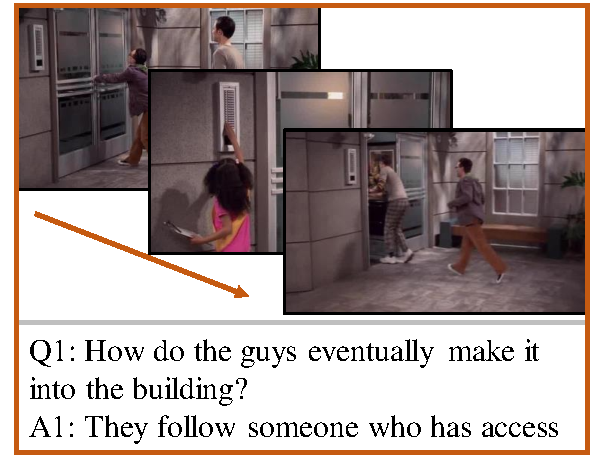
\includegraphics[height=4.2cm]{figure/c2_q1.pdf}
\subcaption{基于全局视觉内容}
\label{fig:c2_diversity_q1} 
\end{subfigure}
\begin{subfigure}[b]{0.35\linewidth}
\centering
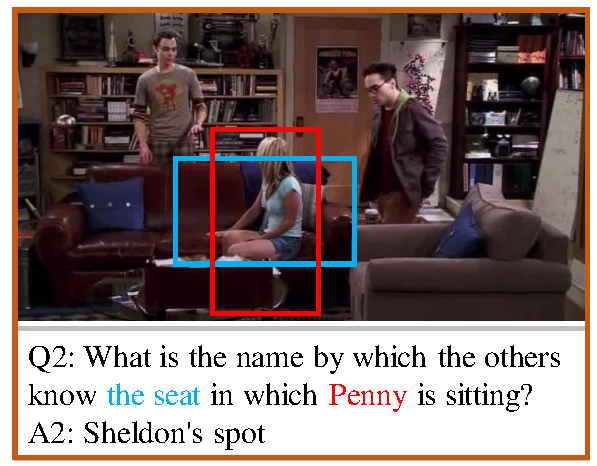
\includegraphics[height=4.2cm]{figure/c2_q2.pdf}
\subcaption{基于细粒度视觉内容}
\label{fig:c2_diversity_q2} 
\end{subfigure}
\begin{subfigure}[b]{0.285\linewidth}
\centering
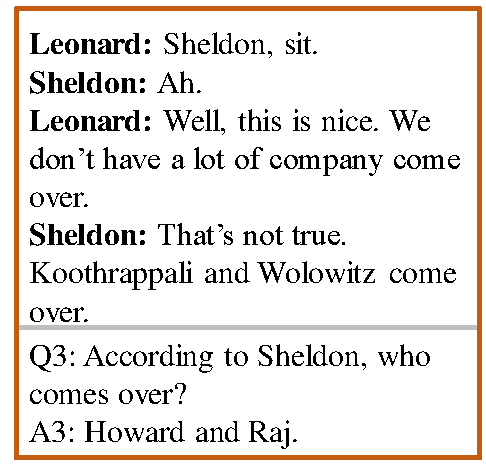
\includegraphics[height=4.2cm]{figure/c2_q3.pdf}
\subcaption{基于语言内容}
\label{fig:c2_diversity_q3} 
\end{subfigure}
\caption{视频问答举例}
\label{fig:c2_diversity} 
\end{figure}
% ********************************************************************

本章提出基于多粒度视觉语言推理的视频问答方法(\textbf{Li}ghtweight \textbf{V}isual \textbf{L}inguistic \textbf{R}easoning,LiVLR)来实现上述功能。
该方法的核心思路是利用图统一视觉和语言的多尺度编码及多样性表征的整合。
具体来说,LiVLR首先使用基于图的视觉编码器和语言编码器在不同的语义层面分别对视频的视觉内容和语言内容进行同程度的编码,生成多粒度的视觉和语言表征。
随后,将获得的多粒度视觉和语言表征以及问题表征传递到专门设计的多样性感知的视觉语言推理模块进行整合。
该模块用多粒度的视觉和语言表征作为初始节点表征构建了一个多样性感知图,其中初始节点表征首先与问题表征进行关联,然后通过不同表征的可学习指数嵌入来增强初始节点表征。
在可学习嵌入的推动下,多样性感知的视觉语言推理模块可以有效地提示不同类型表征之间的差异并调整其重要性;在使用图卷积网络获得答案预测的联合表征时,也可以灵活地对不同的问题做出反应。

本章的主要贡献概括如下:
\begin{itemize}
\item 提出了一种基于多粒度视觉语言推理的视频问答方法。该方法在不同尺度上同程度地编码视频的视觉和语言内容,不仅极大减少了模型参数量还显著提高了对视频中语言信息的利用率。
\item 提出了一种多样性感知的视觉语言推理模。该模块在多粒度视觉语言表征整合时可以有效地保持不同表征的判别性并自适应地学习不同表征的重要性,以应对多种多样的问题。
\end{itemize}



% **************************************************************************
\xsection{预备知识}{Preliminary} 

本节首先描述了视频问答任务的正式定义;然后介绍了本章所提视频问答方法LiVLR的输入,即预提取的视觉和语言特征;最后介绍LiVLR中使用的基本模块,即图注意网络。


\xsubsection{任务的表述}{Problem Definition}
给定视频的视觉内容$\mathit{V}$、语言内容$\mathit{L}$、视频内容相关的问题$\mathit{q}$、以及可能的答案集合$\mathbb{A}$,视频问答模型旨在输出问题的正确答案$\tilde{a}$。即视频问答任务可以表述为:
\begin{equation} 
\tilde{a} = \underset{a \in \mathbb{A}}{\arg \max}~p_{\thetav}\left(a \mid q,\mathit{V}, \mathit{L}\right), 
\end{equation} 
式中,$\thetav$表示可训练的模型参数。


\xsubsection{视觉输入}{Visual Input}
对于每个视频片段,本章采样$N_f$帧的图像并以三种形式表示这些采样的图像以作为本章LiVLR的输入: 
($i$) 图像级的外观特征$[\av_{1}^{0}, \dots, \av_{N_f}^{0}] \in \mathbb{R}^{N_f \times \text{2048}}$; ($ii$) 物体级的区域特征$[\Omat_{1}^{0}, \dots, \Omat_{N_f}^{0}] \in \mathbb{R}^{N_f \times N_o \times \text{2048}}$, 其中$N_o$是单帧图像中物体的数量,且$\Omat_f^{0}$ = $[\ov_1^{0}, \dots, \ov_{N_o}^{0}] \in \mathbb{R}^{N_o \times \text{2048}}, 1\leq f\leq N_f$;($iii$) 短语级物体类别属性特征$[\Cmat_{1}^{0}, \dots, \Cmat_{N_f}^{0}]\in \mathbb{R}^{N_f \times N_o \times \text{768}}$,其中$\Cmat_f^{0}$ = $[\cv_1^{0}, \dots, \cv_{N_o}^{0}] \in \mathbb{R}^{N_o \times \text{768}}$表示第$f$帧图像中$N_o$个物体对应的类别属性的短语嵌入。


\xsubsection{语言输入}{Linguistic Input}
对于每个给定的问题,本章为其提取了token级的特征$\Qmat^{0}$ = $[\qv_1^{0}, \dots, \qv_{N_t}^{0}] \in \mathbb{R}^{N_t \times \text{768}}$,其中$N_t$表示该问题句子中token的数量。除了给定的问题之外,每个视频片段还有$N_s$个对应的语言描述的句子。因此,本章还为这$N_s$个句子提取了相关的语言特征$[\Lmat^{0}_{1}, \dots, \Lmat^{0}_{N_s}] \in \mathbb{R}^{N_s\times N_t\times \text{768}}$,其中$\Lmat_s^{0}$ = $[\lv_1^{0}, \dots, \lv_{N_t}^{0}] \in \mathbb{R}^{N_t \times \text{768}}, 1\leq s\leq N_s$。


\xsubsection{图注意网络}{Attention-Based Graph Convolutional Network}
对于图$\mathcal{G} = (\mathcal{V}, \mathcal{E})$,其中$\mathcal{V} = \{v_1, ..., v_{N_v}\}$表示图节点的集合、$N_v = |\mathcal{V}|$表示节点个数、$\mathcal{E}$表示边的集合、$\Vmat = [\vv_1, \dots, \vv_{N_v}] \in \mathbb{R}^{N_v\times d}$表示初始节点表征的集合,则第$l$层图注意网络中节点$i$的更新公式可以表示为:
\begin{equation}
\vv_i^{(l+1)} = \sigma (\vv_i^{(l)} + \sum_{\vv_j \in \mathcal{N}_i} \alpha_{i,j} \cdot \Wmat^{(l)} \vv_j^{(l)}), 
\label{eq:attention_gcn}
\end{equation}
式中,$\sigma$表示ReLU激活函数;$~\mathcal{N}_i$表示由$\mathcal{E}$确定的节点$i$的邻居节点的集合;$~\Wmat^{(l)} \in \mathbb{R}^{d \times d}$表示第$l$层图神经网络中节点$i$的表征变换矩阵。注意力系数$\alpha_{i, j}$的定义如下:
\begin{equation} 
\alpha_{i, j} = \frac{\exp((\Wmat_q \vv_i)^{\Transpose} \cdot \Wmat_k \vv_j)}{\sum_{\vv_j \in \mathcal{N}_i}\exp((\Wmat_q \vv_i)^{\Transpose} \cdot \Wmat_k \vv_j)},
\label{eq:attn_factor}
\end{equation}
式中,$\Wmat_q \in \mathbb{R}^{d \times d}$和$\Wmat_k \in \mathbb{R}^{d \times d}$是可学习的变换矩阵。


% **************************************************************************
\xsection{视觉语言推理框架}{Visual-Linguistic Reasoning Framework} 
如图~\ref{fig:c2_framework}所示,本章提出的基于多粒度视觉语言联合推理的视频问答方法LiVLR包含视觉编码器、语言编码器、问题编码器、多样性感知的视觉语言推理(\textbf{D}iversity-\textbf{a}ware \textbf{V}isual \textbf{L}inguistic reasoning,DaVL)模块和答案预测模块。
概括来说,LiVLR首先利用基于图的视觉和语言编码器对视觉和语言输入进行多层次编码,生成多粒度的视觉和语言表征。随后,LiVLR通过DaVL模块将获得的多粒度视觉和语言表征进行整合,并生成用于答案预测的联合表征。本节依次介绍上述模块。


% ********************************************************************
\begin{figure*}[!t]
\centering
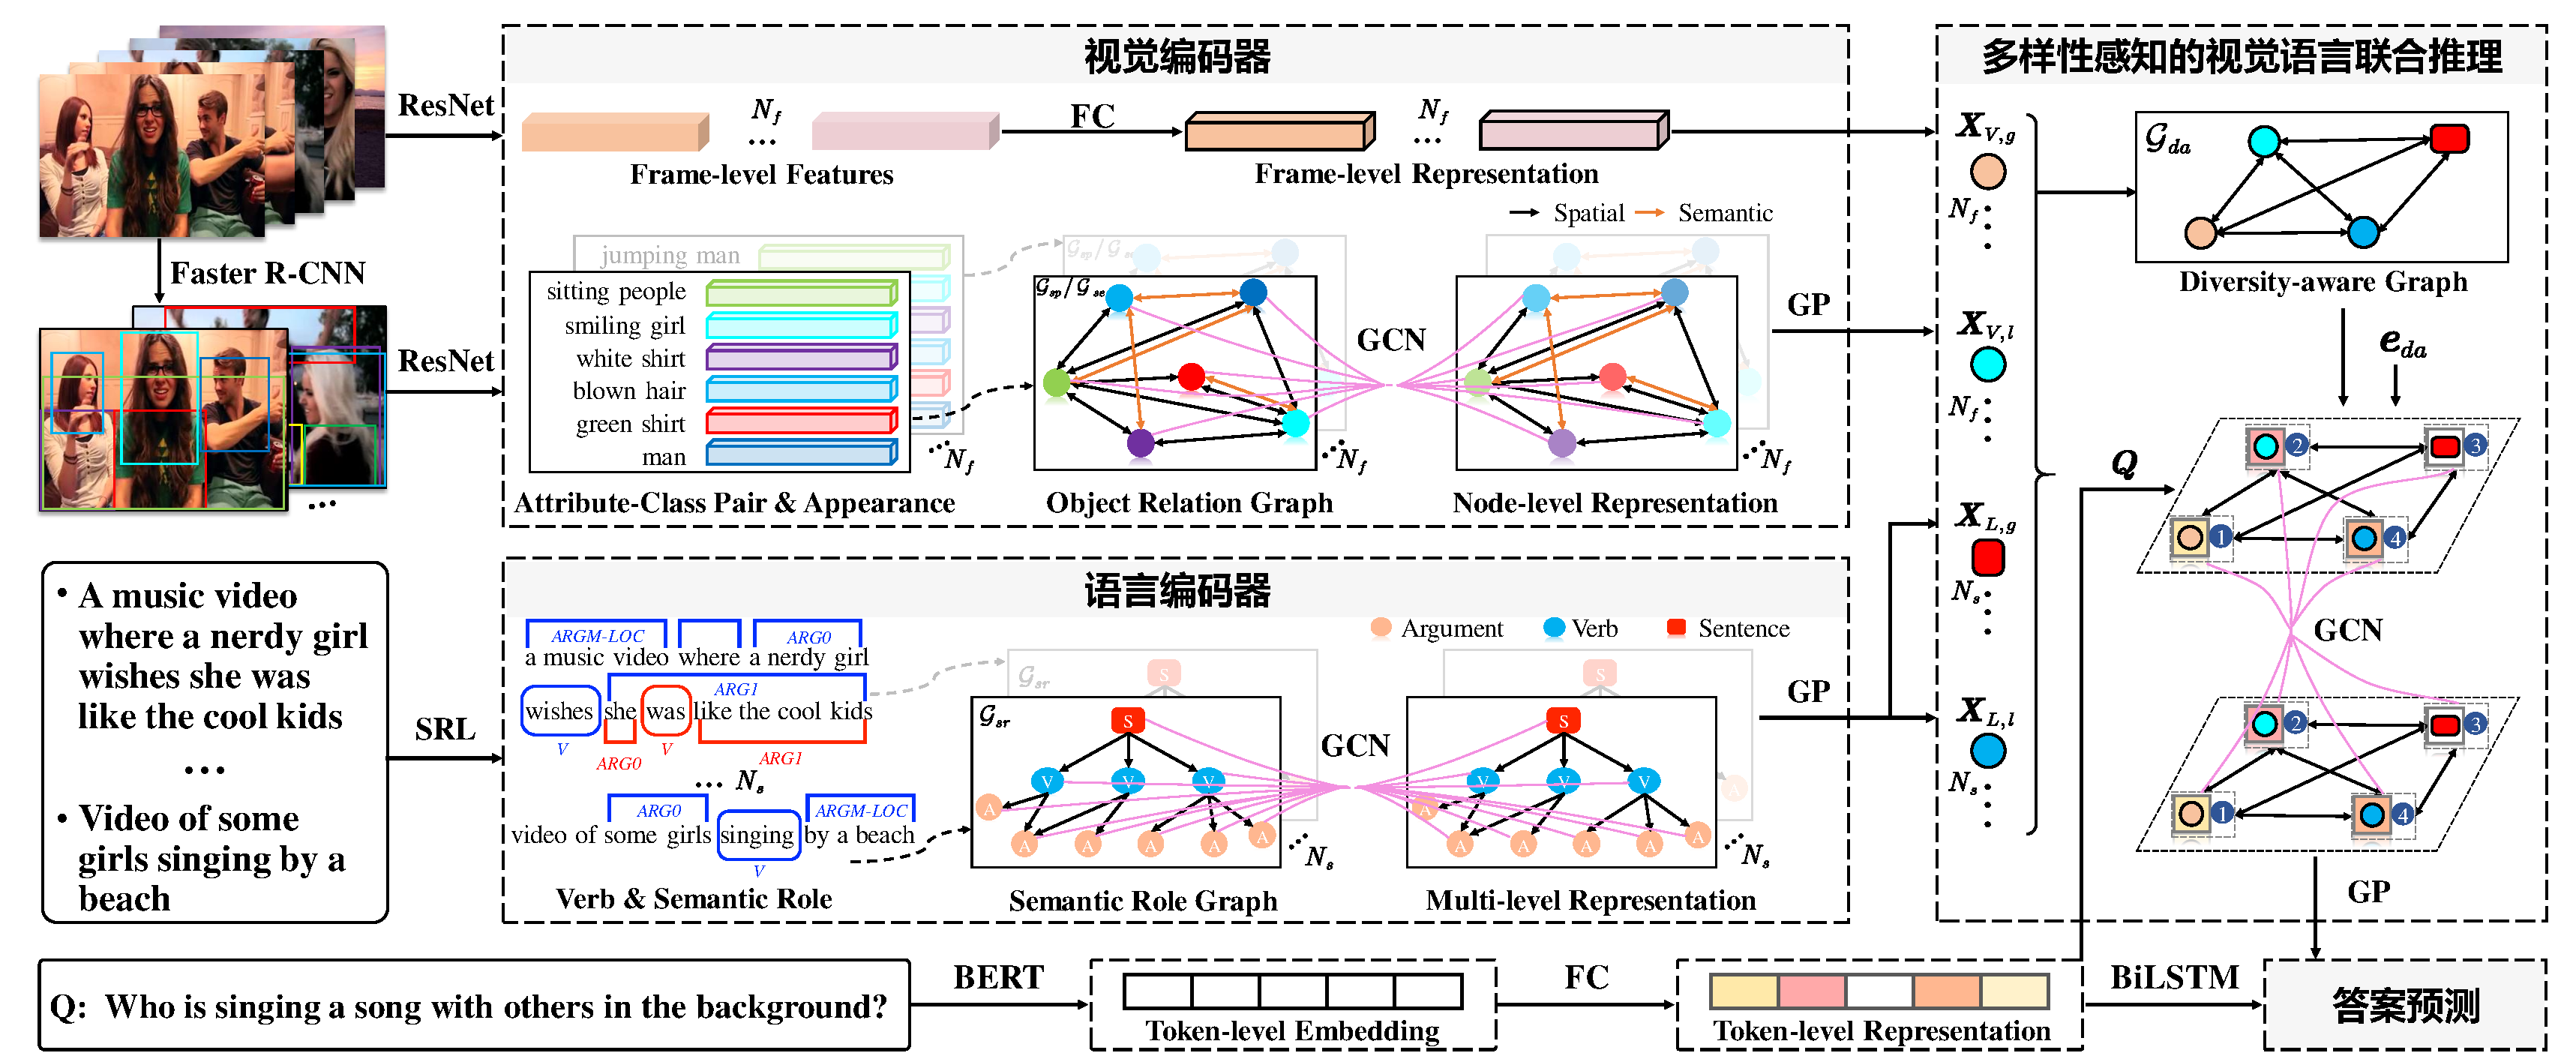
\includegraphics[width=1.0\linewidth]{figure/c2_frame.pdf}
\caption{基于多粒度视觉语言联合推理的视频问答方法的框图}
\label{fig:c2_framework}
\end{figure*}
% ********************************************************************


\xsubsection{视觉编码器}{Visual Encoder}
视觉编码器对视频整体的和细粒度的视觉内容分别编码。具体来说,
对每一个视频片段,为获得整体视觉表征$\Xmat_{V, g}=[\av_1,\dots,\av_{N_f}]\in \mathbb{R}^{N_f \times d}$,本章使用全连接层(FC)将图像级的外观特征$[\av_1^{0}, \dots, \av_{N_f}^{0}]$映射到$d$维空间。为了获得细粒度的视觉表征,本章对物体间细粒度的关系进行编码。
具体过程如下:


\subsubsection{物体关系图构建}
直觉上视觉关系包含反映物体相对位置的空间关系和描述视觉概念语义一致性的语义关系。如图~\ref{fig:c2_framework}所示,对于采样的第$f$帧图像,本章以图像中的物体为节点分别构建空间图$\mathcal{G}_{sp} = (\mathcal{V}, \mathcal{E}_{sp}, \mathcal{R}_{sp})$和语义图$\mathcal{G}_{se} = (\mathcal{V}, \mathcal{E}_{se})$,其中$\mathcal{R}_{sp}$表示边类型的集合。


\subsubsection{物体关系图嵌入}
为了更好地表示物体间的空间和语义关系,本章分别使用位置特征和类别属性特征来增强图$\mathcal{G}_{sp}$ 和 $\mathcal{G}_{se}$的节点嵌入。
具体来说,对于图$\mathcal{G}_{sp}$,给定第$f$帧图像中物体$i$的位置特征为$\pv_i = [p_x, p_y, p_x + p_w, p_y + p_h, p_w, p_h]^{\Transpose}$,其中$(p_x, p_y)$是物体边框的左上坐标、$p_w$和$p_h$分别是物体边框的宽和高,以及第$f$帧图像中物体$i$的区域特征$\ov_i^{0}$,则$\mathcal{G}_{sp}$中第$i$个节点嵌入的初始化为
\begin{align}
\vv_{sp,i}^{(0)} = \Wmat_{sp}^{(0)}([\Wmat_o\ov_i^{0} + \bv_o; \Wmat_{p} \pv_i + \bv_p]), 
\label{eq:sp_init}
\end{align}
式中,上标0表示未进行图编码的初始输入;$[\cdot; \cdot]$表示表征的串联操作;$\Wmat_{o} \in \mathbb{R}^{\text{2048} \times d}$和$\bv_o \in \mathbb{R}^{d}$将预提取的物体级的特征$\ov_i^{0}$映射为$d$维表征;$\Wmat_{p} \in \mathbb{R}^{\text{6} \times d}$和$\bv_p \in \mathbb{R}^{d}$将位置特征$\pv_i$映射为$d$维表征;$\Wmat_{sp}^{(0)} \in \mathbb{R}^{2d\times d}$将串联的物体特征和位置特征映射到$d$维空间。
对于图$\mathcal{G}_{se}$,给定第$f$帧图像中物体$i$的类别属性特征$\cv^{0}_i$,则$\mathcal{G}_{se}$中第$i$个节点嵌入的初始化可以表述成为
\begin{align}
\vv_{se,i}^{(0)} = \Wmat_{se}^{(0)}([\Wmat_o\ov_i^{0} + \bv_o; \Wmat_{c} \cv_i^{0} + \bv_c]), 
\end{align}
式中,$\Wmat_{o}$和$\bv_o$的含义同公式~\eqref{eq:sp_init};$\Wmat_{c} \in \mathbb{R}^{\text{768} \times d}$和$\bv_c \in \mathbb{R}^{d}$将$\cv_i^{0}$映射到$d$维空间;$\Wmat_{se}^{(0)} \in \mathbb{R}^{2d\times d}$将串联后的特征映射到$d$维空间。


\subsubsection{物体关系图编码}
为了将已知边的类型信息$\mathcal{R}_{sp}$引入到图$\mathcal{G}_{sp}$中,本章改进了节点信息聚合公式~(\ref{eq:attention_gcn}),改进后的公式表述如下:
\begin{equation}
\vv_{sp, i\leftarrow j}^{(l)} = \Wmat_{sp}^{(l)} \vv_{sp, j}^{(l)} \oplus \bv_{sp}^{(l)}(r_{i,j}),
\end{equation} 
式中,$\Wmat_{sp}^{(l)} \in \mathbb{R}^{d \times d}$和$\bv_{sp}^{(l)} \in \mathbb{R}^{11}$分别为节点变化矩阵和边类型的可学习向量;$\oplus$表示逐元素加法;$r_{i,j} \in \mathcal{R}_{sp}$表示节点$i$和$j$之间边的类型;$\bv_{sp}^{(l)}(r_{i,j})$表示$\bv_{sp}^{(l)}$中第$r_{i,j}$个元素。
对于图 $\mathcal{G}_{se}$,本章利用图学习器~\cite{norcliffe2018learning} 隐式地学习图像中物体间的语义关系。具体来说,图$\mathcal{G}_{se}$的连接矩阵$\Amat_{se}$可由初始的节点嵌入$\Vmat_{se}^{(0)}$ = $[\vv_{se,1}^{(0)}, \dots, \vv_{se,N_o}^{(0)}] \in \mathbb{R}^{N_o \times d}$按公式~(\ref{eq:graph_learner}) 生成。该公式的具体表述如下:
\begin{equation}
\Amat_{se} = (\Wmat_1 \Vmat_{se}^{(0)}) (\Wmat_2 \Vmat_{se}^{(0)})^{\Transpose},
\label{eq:graph_learner}
\end{equation}
式中,$\Wmat_1, \Wmat_2 \in \mathbb{R}^{d \times d}$为节点变换矩阵。本章还采用了排序策略来约束图的稀疏性,即,本章只保留$\Amat_{se}$每一行的前$N_n$个最大值。在确定连接矩阵后,语义图$\mathcal{G}_{se}$的节点表征按公式~(\ref{eq:attention_gcn})进行更新。
至此,对于视频片段中的第$f$帧图像,本章获得了两种节点级别的表征:$\Vmat_{sp}$ = $[\vv_{sp, 1}, \dots$ $, \vv_{sp, N_o}] \in \mathbb{R}^{N_o\times d}$和$\Vmat_{se}$ = $[\vv_{se, 1}, \dots, \vv_{se, N_o}] \in \mathbb{R}^{N_o\times d}$。最后,本章利用图池化操作生成图级别的表征:$\bar{\vv}_{sp, f}\in \mathbb{R}^d$和$\bar{\vv}_{se, f}\in \mathbb{R}^d$。将$N_f$个图级别的表征堆叠即可获得最终的细粒度的视觉表征$\Xmat_{V, l}$ = $[\xv_1, \dots, \xv_{N_f}]\in \mathbb{R}^{N_f \times d}$,其中$\xv_f=\bar{\vv}_{sp,f} + \bar{\vv}_{se,f}$。


\xsubsection{语言编码器}{Linguistic Encoder}
\label{subsec:c2_srg}
对于一个给定的视频片段,有$N_s$个与之对应的语言句子。本章为每个句子构建一个语义角色图。其中语义角色图的节点包括描述整体事件的句子本身,以及句子中反映细粒度语义一致性的语言成分。
因此,语言编码器对整体和细粒度的语言内容进行统一编码。
具体的编码过程如下:

\subsubsection{语义角色图构建}
为了对第$s$ ($1 \le s \le N_s$)个语言描述的句子构建语义角色图,本章利用现有的语义角色标注(Semantic Role Labeling,SRL)工具~\cite{shi2019simple} 自动生成句子的谓词 (predicate)和论元(arguments)并用语义角色(role)描述谓词论元之间的关系。
本章使用第$s$个句子本身和$N_r$个句子成分构建了语义角色图$\mathcal{G}_{sr}=(\mathcal{V}, \mathcal{E}, \mathcal{T}_{sr})$,其中$|\mathcal{V}|=N_r + 1$、$\mathcal{T}_{sr}$表示节点类型的集合。$\mathcal{G}_{sr}$是有向异构图。在该图中$s$句子本身为作为全局事件节点、谓词和论元分别作为局部的动作节点和实体节点。动作节点直接与事件节点相连,实体节点则根据与动作节点相关的语义角色类型与不同的动作节点相连。

\subsubsection{语义角色图嵌入}
对于$\mathcal{G}_{sr}$,本章使用$s$句子嵌入$\lv \in \mathbb{R}^{d}$初始化全局的事件节点。而为获得$\lv$,本章先使用一个全连接层将$s$句子的token级别的特征$\Lmat_s^{0}$映射到$d$维空间($\Lmat_s\in \mathbb{R}^{N_t \times d}$)。然后,本章利用一个一层的BiLSTM~\cite{hochreiter1997long}对$\Lmat_s$进行编码得到$\lv$,过程如下:
\begin{equation}
\begin{aligned} 
\lv = [\BiLSTM(\overrightarrow{\Lmat_s}; \overrightarrow{\theta_l}); \BiLSTM(\overleftarrow{\Lmat_s}; \overleftarrow{\theta_l})], 
\label{eq:gse_bilstm}
\end{aligned}
\end{equation}
式中,$\overrightarrow{\theta_l}$ ($\overleftarrow{\theta_l}$)为前向(反向)学习参数;$[\cdot; \cdot]$表示特征串联操作。
动作和实体节点则利用非线性变换后的token级别的特征进行初始化,过程如下:
\begin{equation} 
\vv_{sr, i}^{(0)} = \Wmat_{sr}^{(0)} \lv_{t \leftrightarrow i}^{0}, ~~2 \le i \le N_r + 1, 
\end{equation} 
式中,$\lv_{t \leftrightarrow i}^{0} \in \Lmat_s^{0}$是指$i$节点表示的谓词或论元对应的token级别的表征。$\Wmat_{sr}^{(0)}\in \mathbb{R}^{\text{768} \times d}$的作用是将特征映射到$d$维空间。
因为语义角色本身就蕴涵着动作节点和实体节点之间的关系,所以本章将语义角色类型引入到$\mathcal{G}_{sr}$。具体来说,本章使用角色嵌入对$i$节点进行增强,过程表述如下:
\begin{equation}
\tilde{\vv}_{sr,i}^{(l)} = \vv_{sr,i}^{(l)} \odot \Wmat_{sr}^{(l)}[t_{sr, i}, :], ~2 \le i \le N_r + 1, 
\end{equation}
式中,$\odot$表示逐元素乘法;$\Wmat_{sr}^{(l)} \in \mathbb{R}^{N_r \times d}$表示可学习的角色嵌入矩阵;$\Wmat_{sr}^{(l)}[t_{sr, i}, :]$表示矩阵$\Wmat_{sr}^{(l)}$的第$t_{sr, i}$行。


\subsubsection{语义角色图编码}
在图$\mathcal{G}_{sr}$中,本章采用基于注意力的图神经网络来编码的节点间的语义关联。具体来说,本章首先采用公式~(\ref{eq:attn_factor})中描述的注意机制来刻画不同层次节点的语义关系。然后使用公式~(\ref{eq:attention_gcn})更新$i$节点的表征。
在对图$\mathcal{G}_{sr}$进行编码后,可以获得该图对应的事件节点表征$\vv_{sr, 1}$。$N_s$个事件表征堆叠即为语言编码器生成的整体的语言表征$\Xmat_{L, g}\in \mathbb{R}^{N_s\times d}$。
而为获得$N_s$个句子的细粒度语言表征,本章首先采用图池化操作对图$\mathcal{G}_{sr}$中动作和实体节点表征求平均值$\bar{\vv}_{sr, s}\in \mathbb{R}^d$,该值即为第$s$个句子的细粒度表征。然后堆叠$N_s$个语义角色图的池化表征即可得到语言编码器生成的细粒度语言表征$\Xmat_{L, l} \in \mathbb{R}^{N_s \times d}$。


\xsubsection{多样性感知的视觉语言推理}{Diversity-Aware Visual-Linguistic Reasoning Module}

为了更好地融合多粒度的视觉和语言表征,本章不仅需要在表征整合时兼顾表征的多样性,还需要在不同的语义层面上对视觉和语言表征进行对齐(例如, 句子 $\leftrightarrow$ 图像、语义角色 $\leftrightarrow$ 物体实例)。
因此,本章提出使用视觉编码器和语言编码器输出的多粒度视觉和语言表征构建具有多样性感知的异构图,并利用图神经网络模块来进一步编码和捕捉节点间的关系。


\subsubsection{多样性感知图构建}
为了以多样性感知的方式整合已经获得的多粒度视觉和语言表征,本章构建了无向异构图$\mathcal{G}_{da}$。图$\mathcal{G}_{da}$包含四种类型的节点:$N_f$个图像级别的节点、$N_f$个物体级别的节点、$N_s$个句子级别的节点和$N_s$个语义角色级别的节点。


\subsubsection{多样性感知图嵌入}
为获得多样性感知的图嵌入,本章首先使用注意力模块将已经获得的多粒度视觉和语言表征$\{\Xmat_{V, g}, \Xmat_{V, l}, \Xmat_{L, g}, \Xmat_{L, l}\}$与问题进行关联。具体来说,本章分别应用多头注意力~\cite{vaswani2017attention}于这四种表征上,该过程表述如下:
\begin{equation}
\begin{aligned}
&\mathcal{Q}_{\text{att}}(\Xmat, \Qmat) = \bigcup_{h=1}^{N_h} \Wmat_h \sigma \left(\frac{\Wmat_h^q\Xmat(\Wmat_h^k \Qmat)^{\Transpose}}{\sqrt{d_k/N_h}}\right) \Wmat_h^v \Qmat, 
\label{eq:alpha_ij}
\end{aligned}
\end{equation} 
式中,$\Xmat \in \{\Xmat_{V, g}, \Xmat_{V, l}, \Xmat_{L, g}, \Xmat_{L, l}\}$;$\Qmat \in \mathbb{R}^{N_t \times d}$是利用非线性操作将$\Qmat^{0}$映射到$d$维空间后的token级别的问题嵌入;$\cup$表示表征的串联操作;$N_h$是多头注意力中的头数;$\sigma$表示softmax激活函数;$d_k$是缩放因子;$\Wmat_q^h, \Wmat_k^h, \Wmat_v^h \in \mathbb{R}^{d/N_h \times d}$和$\Wmat_x \in \mathbb{R}^{d \times d/N_h}$是参数矩阵。
注意力模块输出的问题关联后的多粒度视觉语言表征就是图$\mathcal{G}_{da}$的初始节点表征$\Vmat^{0} \in \mathbb{R}^{(2N_f + 2N_s) \times d}$。
此外,为了在表征整合中注入多粒度视觉和语言表征的多样性感知信息,本章使用不同类型表征的索引嵌入来增强初始节点表征。索引嵌入矩阵是可学习的,可用于动态调整不同类型节点的重要性。对于$i$节点,节点增强的过程如下:
\begin{equation} 
\tilde{\vv}_{da, i}^{(0)} = \vv_{da, i}^{(0)} \odot \Wmat_{da}^{(0)}[g_i, :],
\end{equation}
式中,$\Wmat_{da}^{(0)} \in \mathbb{R}^{4 \times d}$就是索引嵌入的变换矩阵;$g_i \in \{1, ..., 4\}$表示$\{\Xmat_{V, g}, \Xmat_{V, l}, \Xmat_{L, g}, \Xmat_{L, l}\}$的索引;$\Wmat_{da}^{(0)}[g_i, :]$表示$\Wmat_{da}^{(0)}$的第$g_i$行。


\subsubsection{多样性感知图编码}
本章使用经典图神经网络编码图$\mathcal{G}_{da}$,对于图$\mathcal{G}_{da}$中的$i$节点,表征更新公式如下:
\begin{equation}
\vv_{da, i}^{(l+1)} = \ReLU (\tilde{\vv}_{da, i}^{(l)} + \sum_{\tilde{\vv}_{da, j} \in \mathcal{N}_i} \Wmat_{da}^{(l)} \tilde{\vv}_{da, j}^{(l)}),
\label{eq:da_GCN}
\end{equation}
式中,$\mathcal{N}_i$表示$i$节点的邻居;$\Wmat_{da}^{(l)}\in \mathbb{R}^{d\times d}$是节点表征的变换矩阵。
在利用DaVL对多粒度视觉语言和表征进行有效编码之后,本章对图$\mathcal{G}_{da}$执行图池化操作得到最终用于答案预测的联合表征$\hat{\xv} = \bar{\vv}_{da} \in \mathbb{R}^d$。


% **************************************************************************
\xsubsection{问题编码器}{Question Encoder}
本章使用一层的BiLSTM~\cite{hochreiter1997long}编码$\Qmat$获得句子级别的问题表征$\hat{\qv} \in \mathbb{R}^d$:
\begin{equation}
\begin{aligned}
\hat{\qv} &= [\BiLSTM(\overrightarrow{\Qmat}; \overrightarrow{\theta_q}); \BiLSTM(\overleftarrow{\Qmat}; \overleftarrow{\theta_q})], 
\label{eq:q_bilstm}
\end{aligned}
\end{equation}
式中,$\overrightarrow{\hv_q}$和$\overleftarrow{\hv_q}$分别是前向和反向隐藏层状态;$\overrightarrow{\theta_q}$和$\overleftarrow{\theta_q}$是参数矩阵。


% **************************************************************************
\xsubsection{答案预测}{Answer Prediction}

\subsubsection{多选式视频问答}
在多选式视频问答的设置中,正确答案从$N_k$个候选答案中选择。这时,本章首先使用一层的BiLSTM~\cite{hochreiter1997long}生成候选答案的嵌入表征$\{\hat{\ev}_k|1 \leq k \leq N_k\}$。然后,本章将$\hat{\xv}$, $\hat{\qv}$和$\hat{\ev_k}$传入线性回归器($\mathcal{M}_{\text{reg}}$)中去输出每个候选答案的得分:
\begin{equation}
\begin{aligned}
s_k = \mathcal{M}_{\text{reg}}([\hat{\xv}; \hat{\qv}; \hat{\ev_{k}}]), 1 \leq k \leq N_k,  
\end{aligned}
\end{equation} 
式中,正确候选答案的分数$s^p$为正,其余分数$(s_1^n, \dots, s_{N_k -1}^n)$为负。训练时,本章使用合页损失$\sum_{t=1}^{N_k-1}\max (0, 1 - (s^p - s_{t}^n))$。

\subsubsection{开放式视频问答}
在开放式视频问答的设置中,正确答案从预先定义的包含大量答案的集合$\mathbb{A}$中选择。
这时视频问答任务可被视为多标签分类问题,并采用交叉熵损失函数进行训练。
所以,本章将联合表征$\hat{\xv}$和问题表征$\hat{\qv}$传入到由两层全连接层构成的分类器($\mathcal{M}_{\text{cls}}$)中去计算答案概率:
\begin{equation}
\begin{aligned}
\yv_o = \mathcal{M}_{\text{cls}}([\hat{\xv}; \hat{\qv}]), 
\end{aligned}
\end{equation}
式中,$\yv_o \in \mathbb{R}^{|\mathbb{A}|}$。


% **************************************************************************
\xsection{实验及结果分析}{Experiment and Result Analysis}

\xsubsection{实验设置}{Experimental Setting}

\subsubsection{数据集}
本章的实验在MSRVTT-QA~\cite{xu2017video}、KnowIT VQA~\cite{garcia2020knowit}和TVQA~\cite{lei2018tvqa}三个视频问答数据集上完成。
其中,MSRVTT-QA提供与视频内容相关的描述、KnowIT VQA提供字幕和高度结构化的知识、TVQA提供字幕。
LiVLR分别使用提供的的描述、字幕和知识作为的语言输入来生成多粒度的语言表征。
表~\ref{tab:c2_data_statistics}总结了实验数据集的统计信息。
具体来说,MSRVTT-QA包含约10,000个视频片段和243,680个问题-答案对。问题的设置是开放式的,预设答案集合的大小为1000。有What、 Who、 How、 When和Where五种问题类型。
KnowIT VQA是一个小规模的多选式视频问答数据集,由12,087个视频片段和24,282个问题-答案对组成。该数据集为每个问题提供4个候选答案并具有Visual、Textual、Temporal和Knowledge四种问题类型。
TVQA是一个大规模的多选式视频问答数据集,包括来自六个电视节目的21,793个视频片段,以及152,545个问题-答案对。它为每个问题提供了5个候选答案。

\begin{table}[!t]
\caption{数据集的统计信息
% 。LType和QType表示语言内容的类型和问题设置的类型,OE和MC分别表示开放式和多选式视频问答设置。
}
\label{tab:c2_data_statistics} 
\setlength{\tabcolsep}{.89mm}{
% \begin{tabularx}{\textwidth}{l|ccc|ccc|ccc|cc}
\begin{tabularx}{\textwidth}{lccccccccccc}
\toprule
\multirow{2}{*}{Dataset} 
&\multicolumn{3}{c}{\#Question} 
&\multicolumn{3}{c}{\#Video Clip}  
&\multicolumn{3}{c}{\#Sentence} 
&\multirow{2}{*}{LType} 
&\multirow{2}{*}{QType} 
\\

\cmidrule(lr){2-4} 
\cmidrule(lr){5-7}
\cmidrule(lr){8-10}
~&\multicolumn{1}{c}{Train} 
&\multicolumn{1}{c}{Val} 
&\multicolumn{1}{c}{Test} 
&\multicolumn{1}{c}{Train} 
&\multicolumn{1}{c}{Val} 
&\multicolumn{1}{c}{Test} 
&\multicolumn{1}{c}{Train} 
&\multicolumn{1}{c}{Val} 
&\multicolumn{1}{c}{Test} 
& & 
\\
\midrule

MSRVTT-QA~\cite{xu2017video} &158,581 &12,278 &72,821 &6,513 &497 &2,990 &78,156 &5,964 &35,880 
% &64 &\textbf{10} &12 
&caption &OE 
\\
KnowIT-VQA~\cite{garcia2020knowit} &19,569 &2,352 &2,361 &9,731 &1,178 &1,178 &19,569 &2,352 &2,361 
% &\textbf{32} &12 &\textbf{12/1} 
&sub/know &MC 
\\
TVQA~\cite{lei2018tvqa} &122,039 &15,253 &7,623 &17,435 &2,179 &1,089 &17,435 &2,179 &1,089 
% &\textbf{32} &12 &16 
&sub &MC 
\\ 
\bottomrule
\end{tabularx}
}
\end{table}




\subsubsection{评价指标}
本章遵循上述三个视频问答数据集的原始设定,以准确率(Accuracy)为视频问答性能的评价指标。即本文在MSRVTT-QA、KnowIT VQA和TVQA上的评价指标如下:
\begin{equation}
\begin{aligned}
\mathrm{Accuracy} (a) = \InF \{a = \tilde{a}\}, ~a \in \mathbb{A},  
\end{aligned}
\end{equation} 
式中,答案$a$属于答案集合$\mathbb{A}$,$\tilde{a}$表示正确答案;$\InF(\cdot)$表示指示函数,当$\cdot$为真时值为1,反之值为0。


\subsubsection{特征提取细节}
为获得LiVLR的视觉与语言输入,本章使用在ImageNet~\cite{deng2009imagenet}上预训练后的ResNet-101~\cite{he2016deep}为所有数据集提取全局的图像外观特征;
使用在VG~\cite{krishna2017visual}上预训练后的BUA Faster R-CNN~\cite{anderson2018bottom}检测每帧图像中的物体以及物体对应的类别属性。
对于MSRVTT-QA,本章等间隔的从每个视频片段中采样$N_f=64$帧图像并从该视频段对应的视频描述中采样$N_s=12$个语言句子。每帧图像中检测的物体数量为$N_o=10$。
对于KnowIT VQA,采样的图像和检测的物体的数量分别为$N_f=32$和$N_o=12$。本章使用$N_s=12$个原始字幕和从视频字幕中凝练出的$N_s=1$个知识作为语言句子。
对于TVQA,采样的图像和检测的物体的数量分别为$N_f=32$和$N_o=12$。本章使用$N_s=16$个字幕作为语言句子。


\subsubsection{实现细节}
对于LiVLR,本章设置特征维度$d$为512、图神经网络的层数$l$为1、第~\ref{subsec:c2_srg}节中语义角色的个数$N_r$为16、公式~(\ref{eq:graph_learner})中矩阵$\Amat_{se}$保留的最大值$N_n$为5。公式~(\ref{eq:alpha_ij})中head的数量$N_h$在数据集MSRVTT-QA、KnowIT-VQA和TVQA分别被设置为16、 8和16。
本章利用PyTorch深度学习框架,在两张NVIDIA GeForce GTX 2080Ti GPUs上进行了实验。在训练过程中,本章使用AdamW~\cite{loshchilov2017decoupled}优化器训练了80个轮次、初始学习率为$8\times 10^{-5}$、批次大小为256。

\begin{table}[!t]
\caption{在MSRVTT-QA数据集上的性能比较
% 。\#Param表示可训练的模型参数的数量,
% Pretraining提示方法是否采用大规模视频语言预训练。
}
\label{tab:c2_MSRVTT} 
\setlength{\tabcolsep}{2.7mm}{
\begin{tabularx}{\textwidth}{llccccccccc}
\toprule
\multirow{2}{*}{S/N}
&\multirow{2}{*}{Method} 
% &\multicolumn{3}{c|}{Video Representation} 
&\multicolumn{1}{c}{\multirow{2}{*}{\#Param}}
&\multicolumn{1}{c}{\multirow{2}{*}{Pretraining}}
&\multicolumn{6}{c}{Accuracy (\%)} 
\\ 

\cmidrule(l){5-10} 
& 
& &
&What &Who &How &When &Where &All 
\\ 
\midrule

\multirow{4}{*}{({I})}
&SSML~\cite{amrani2021noise} 
% &ResNeXt-101 &ResNet-152 &\xmark 
&- &\checkmark
&- &- &- &- &- &35.1 
\\ 

&ClipBERT~\cite{lei2021less} 
% &\xmark &ResNet-50 &\xmark 
&113.5M &\checkmark 
&- &- &- &- &- &37.4 
\\ 

&CoMVT~\cite{seo2021look} 
% &S3D &\xmark &Faster R-CNN 
&- &\checkmark 
&- &- &- &- &- &39.5 
\\ 

&VQA-T~\cite{yang2021just} 
% &S3D &\xmark &\xmark 
&156.5M &\checkmark 
&- &- &- &- &- &41.5 
\\ 

\midrule

\multirow{6}{*}{({II})} 
&ST-VQA~\cite{jang2017tgif} 
% &C3D &ResNet-152 &\xmark 
&39.0M &\xmark 
&24.5 &41.2 &78.0 &76.5 &34.9 &30.9 
\\

% ST-VQA在MSRVTT数据集上的实验结果来源于[HME]
&Co-mem~\cite{gao2018motion} 
% &BN-Inception &ResNet-152 &\xmark 
&69.5M &\xmark 
&23.9 &42.5 &74.1 &69.0 &42.9 &32.0 
\\

&GRA~\cite{xu2017video} 
% &C3D &VGG16 &\xmark 
&35.4M &\xmark 
&26.2 &43.0 &80.2 &72.5 &30.0 &32.5 
\\

% 通过AMU单元实现 
&HME~\cite{fan2019heterogeneous} 
% &C3D &VGG16 &\xmark 
&48.3M &\xmark 
&26.5 &43.6 &82.4 &76.0 &28.6 &33.0 
\\

&MiNOR~\cite{jin2019multi} 
% &\xmark &VGG16 &Mask R-CNN 
&- &\xmark 
&29.5 &45.0 &83.2 &74.7 &42.4 &35.4 
\\ 

&HCR~\cite{le2020hierarchical} 
% &ResNeXt-101 &ResNet-101 &\xmark 
&43.7M &\xmark 
&- &- &- &- &- &35.6 
\\ 

\midrule

\multirow{6}{*}{({III})}
&MASN~\cite{seo2021attend} 
% &I3D &ResNet-152 &Faster R-CNN 
&28.2M &\xmark 
&- &- &- &- &- &35.2 
\\ 

&HGA~\cite{jiang2020reasoning} 
% &C3D &VGG16 &\xmark 
&121.4M &\xmark 
&29.2 &45.7 &83.5 &75.2 &34.0 &35.5 
\\

&DualVGR~\cite{wang2021dualvgr} 
% &ResNeXt-101 &ResNet-101 &\xmark 
&34.1M &\xmark 
&29.4 &45.6 &79.8 &76.7 &36.4 &35.5 
\\ 

% conditional relation (通过对不同尺度/帧数的feature采样实现relation的表征)
&Bri2Ans~\cite{park2021bridge} 
% &ResNeXt-101 &ResNet-101 &\xmark 
&- &\xmark 
&- &- &- &- &- &36.9 
\\ % GNN for both interaction and fusion 

\rowcolor{gray!15}\cellcolor{white}
&\textbf{LiVLR-V} 
% &\xmark &ResNet-101 &Faster R-CNN 
&10.7M &\xmark 
&34.1 &50.9 &81.5 &\textbf{82.8} &42.2 &40.6 
\\ 
% \cline{2-13}

\rowcolor{gray!15}\cellcolor{white} 
&\multicolumn{1}{l}{\textbf{LiVLR (ALL)}} 
% &\xmark &ResNet-101 &Faster R-CNN 
&15.0M &\xmark 
&\textbf{50.3} &\textbf{77.1} &\textbf{94.2} &81.3 &\textbf{48.4} &\textbf{59.4} 
\\ 
\bottomrule
\end{tabularx}
}
\end{table}
 
\xsubsection{与不同方法的性能比较}{Comparison with State-of-the-Arts}

本章在一个开放式(MSRVTT-QA)和两个多选式(KnowIT VQA和TVQA)视频问答数据集上将本章提出的LiVLR与最先进的方法进行了比较。


\subsubsection{在MSRVTT-QA数据集上的实验}
在MSRVTT-QA数据上,本章主要与最近提出的方法进行了对比。这些方法包括:
Bri2Ans~\cite{park2021bridge}, DualVGR~\cite{wang2021dualvgr}, HGA~\cite{jiang2020reasoning}, MASN~\cite{seo2021attend}, HCR~\cite{le2020hierarchical}, MiNOR~\cite{jin2019multi}, HME~\cite{fan2019heterogeneous}, GRA~\cite{xu2017video}, Co-mem~\cite{gao2018motion}, ST-VQA~\cite{jang2017tgif}, VQA-T~\cite{yang2021just}, CoMVT~\cite{seo2021look}, ClipBERT~\cite{lei2021less}和SSML~\cite{amrani2021noise}。
其中,(I)VQA-T、CoMVT、ClipBERT和SSML采用了大规模的视频语言预训练来提高下游视频问答任务的性能。而通常来说,这种基于预训练的方法性能要优于其它的方法。
(II)ST-VQA, Co-mem, GRA, HME, MiNOR和HCR采用注意机制来实现跨模态表征的交互和融合。
(III)MASN, HGA, DualVGR和Bri2Ans使用了图神经网络来实现表征的交互和融合。
具体来说,MASN采用图神经网络来编码视觉表征;HGA依次应用注意力机制和图神经网络进行表征融合;DualVGR和Bri2Ans 与本章提出的LiVLR最相似,都是利用图神经网络进行表征编码和融合。
上述所有非基于预训练的方法均采用预提取的视觉特征以减少计算和存储代价。


表~\ref{tab:c2_MSRVTT}总结了LiVLR与上述方法在MSRVTT-QA上的性能比较。考虑到所有对比方法都没有使用除给定问题之外的语言信息,为了更公平地进行比较,本章主要将它们与本章提出LiVLR-V进行比较。LiVLR-V即是只使用DaVL整合多粒度视觉表征$(\Xmat_{V, g}, \Xmat_{V, l})$得到最终用于答案预测的表征$\hat{\xv}$。而且,与最好的基于预训练的方法VQA-T相比,本章的LiVLR-V也是有可比性的。
在只是用视觉表征的情况下,本章的方法LiVLR-V的性能已经超过了所有非预训练的方法的性能。而一旦利用了多粒度语言表征$(\Xmat_{L, g}, \Xmat_{L, l})$,本章LiVLR的性能进一步提升了18.8\%。




\subsubsection{在KnowIT VQA数据集上的实验}
在KnowIT VQA数据集上,本章与该数据上当时已有的全部方法进行了对比。这些方法包含ROCK~\cite{garcia2020knowit}、TVQA~\cite{lei2018tvqa}和ROLL~\cite{garcia2020knowledge}。具体来说,ROCK采用了四种不同的技术来描述视频帧的视觉内容:
(\emph{i}) image:使用ResNet50~\cite{he2016deep}提取的图像级别的外观特征;(\emph{ii}) concept:使用BUA Faster R-CNN~\cite{anderson2018bottom}获得的词袋表征及其属性;(\emph{iii}) facial:使用用人脸检测器~\cite{parkhi2015deep}检测出的视频片段中核心人物人脸的词袋表征;(\emph{iv}) caption:使用描述生成器~\cite{xu2015show}生成的描述的表征。
ROLL生成无监督的视频场景描述作为视觉输入。
本章提出的LiVLR使用图像级的外观特征和物体级的区域特征(I + O)作为视觉输入。
实验时,为了获得多粒度的语言表征,本章分别利用数据集提供的$N_s=12$个字幕和$N_s=1$个知识作为本章语言编码器的原始输入。

实验结果如表~\ref{tab:c2_knowit}所示。总的来说,本章提出的LiVLR在KnowIT VQA数据集上的性能优于已有方法,与表现第二好的ROCK方法相比,LiVLR性能提升了大约4\%。
此外,本章发现在使用字幕和知识分别为语言输入时,LiVLR取得的整体性能相似。但在回答Textual类型问题时,使用字幕作为语言输入,LiVLR能取得更好的性能。
可能的原因是对于一个视频-问题对,LiVLR只能从提供的知识句中获得一对多粒度的语言表征,这远远少于获得的多粒度视觉表征的数量,造成视觉信息在表征整合过程中占主导地位,削弱了语言信息的作用。

\begin{table}[!t]
\caption{在KnowIT VQA数据集上的性能比较 
% G(H)表示输入的语言句子是在线生成的knowledge(离线人工标注的knowledge)。
}
\label{tab:c2_knowit}
\setlength{\tabcolsep}{2.199mm}{
\begin{tabularx}{\textwidth}{lccccccccc}
\toprule
\multirow{2}{*}{Method} 
&\multirow{2}{*}{Visual Input} 
&\multicolumn{2}{c}{linguistic Input} 
&\multicolumn{5}{c}{Accuracy (\%)} 
\\ 
\cmidrule(lr){3-4}
\cmidrule(l){5-9}
& &\footnotesize{Subtile} &\footnotesize{Knowledge} 
&\footnotesize{Visual} &\footnotesize{Textual} &\footnotesize{Temporal} &\footnotesize{Knowledge} &\footnotesize{All} 
\\
\midrule 
% Human &- &96.1 &93.6 &85.7 &86.7 &89.6 \\ 
% \hline 
TVQA\cite{lei2018tvqa} &concept &\checkmark &\xmark 
&61.2 &64.5 &54.7 &46.6 &52.2 \\ 
ROCK\cite{garcia2020knowit} &image &\checkmark &G 
&65.4 &68.1 &62.8 &64.6 &65.2 
\\ 
ROCK\cite{garcia2020knowit} &concept &\checkmark &G 
&65.4 &68.5 &62.8 &64.6 &65.2 
\\
ROCK\cite{garcia2020knowit} &facial &\checkmark &G 
&65.4 &68.8 &62.8 &64.6 &65.2 
\\
ROCK\cite{garcia2020knowit} &caption &\checkmark &G 
&64.7 &67.8 &59.3 &64.3 &64.6 
\\
ROLL\cite{garcia2020knowledge} &description &\checkmark &G 
&71.8 &73.9 &64.0 &71.3 &71.5 
\\

\midrule

ROLL~\cite{garcia2020knowledge} &description &\checkmark &H 
&70.8 &75.4 &57.0 &56.7 &62.0 
\\
ROCK\cite{garcia2020knowit} &concept &\checkmark &H 
&74.7 &\textbf{81.9} &75.6 &70.8 &73.1 
\\
\rowcolor{gray!15} \textbf{LiVLR} &I + O &\checkmark &\xmark 
&76.4 &75.1 &72.2 &77.3 &77.0 
\\ 
\rowcolor{gray!15} \textbf{LiVLR} &I + O &\xmark &H 
&\textbf{79.3} &70.5 &\textbf{76.4} &\textbf{78.0} &\textbf{77.1} 
\\ 
\bottomrule
\end{tabularx}
}
\end{table}

 


\subsubsection{在TVQA数据集上的实验}
在TVQA数据集上,本章主要与该数据上当时已有的方法,即 Multi-Stream~\cite{lei2018tvqa}、MSAN~\cite{kim2020modality}、PAMN~\cite{kim2019progressive} 和 STAGE~\cite{lei2020tvqa} 进行比较。
所有对比方法和本章的方法一样均使用视频片段的视觉内容和与之对应的语言内容即字幕进行答案预测。
在TVQA验证集上的性能比较如表~\ref{tab:c2_tvqa}所示。
由表中的实验结果本章可以发现与表中的这两类方法(即,该类方法使用或不使用TVQA数据集提供的时间戳注释)相比,本章所提出的LiVLR在不使用时间戳注释的情况下取得了该数据上当时最优的性能。

\begin{table}[!t]
\centering
\caption{在TVQA数据集上的性能比较 
% Timestamp提示方法是否利用数据集提供的时间戳。
} 
\label{tab:c2_tvqa} 
\setlength{\tabcolsep}{23.95mm}{
\begin{tabularx}{\textwidth}{@{}lcc}
\toprule
~Method &Timestamp &Accuracy (\%) 
\\
\midrule
~Multi-Stream~\cite{lei2018tvqa} &\checkmark &68.85 
\\
~MSAN~\cite{kim2020modality} &\checkmark &71.62 
\\
\midrule

~Multi-Stream~\cite{lei2018tvqa} &\xmark &65.85 
\\
~PAMN~\cite{kim2019progressive} &\xmark &66.38 
\\
~MSAN~\cite{kim2020modality} &\xmark &69.89 
\\ 
~STAGE~\cite{lei2020tvqa} &\xmark &70.50 
\\
% \rowcolor{gray!15} 
~\textbf{LiVLR} &\xmark &\textbf{73.95} 
\\
\bottomrule
\end{tabularx} 
}
\end{table} 


\subsubsection{在MSRVTT-QA数据集上模型参数和精度的对比}
图~\ref{fig:c2_param_acc} 展示了在MSRVTT-QA数据集上本章提出的LiVLR-V与已有视频问答模型在参数量和精度层面的比较。
从图中的结果本章可以发现,本章提出的LiVLR-V在具有最少参数量的情况下取得了第二的性能,
而性能第一的方法VQA-T是基于预训练的方法,模型参数量较本章提出的方法高一个数量级(10.7M vs. 156.5M)。



% ********************************************************************
\begin{figure}[!t]
\centering
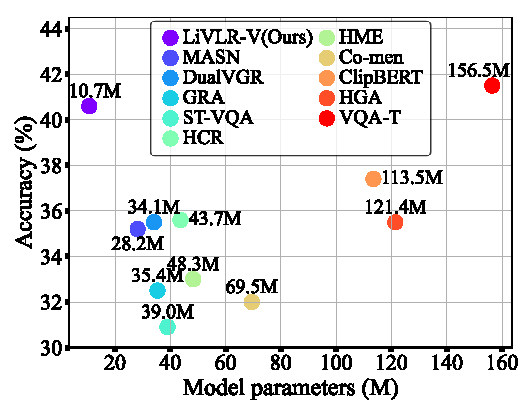
\includegraphics[width=0.55\linewidth]{figure/c2_F2.pdf}
\caption{在MSRVTT-QA数据集上模型参数量和精度的对比}
\label{fig:c2_param_acc}
\end{figure}
% ********************************************************************


\xsubsection{消融实验}{Ablation Study}
\label{sec:c2_ab_all}

为了验证LiVLR各核心组件的有效性和影响,本章在MSRVTT-QA和KnowIT-VQA数据集上进行了消融实验。
对于KnowIT-VQA数据集,本章使用数据集提供的知识提取多粒度语言表征。

\subsubsection{表征整合方法DaVL的有效性}
在LiVLR中,DaVL用于更好地整合多粒度的视觉和语言表征。为了评价其有效性,本章比较了提出的DaVL和其它三种表征整合方法:
$\blacktriangleright$RI-GCN:使用初始版本的图神经网络整合获得的问题相关的多粒度视觉语言表征\{$\Xmat_{V, g}, \Xmat_{V, l}, \Xmat_{L, g}, \Xmat_{L, l}$\}$^q$;
$\blacktriangleright$RI-AT:使用co-attention操作整合\{$\Xmat_{V, g}, \Xmat_{V, l}, \Xmat_{L, g}, \Xmat_{L, l}$\}$^q$;
$\blacktriangleright$RI-Concat:使用向量串联操作整合\{$\Xmat_{V, g}, \Xmat_{V, l}, \Xmat_{L, g}, \Xmat_{L, l}$\}$^q$。
三种表征整合的对比方法中RI-GCN与本章提出的DaVL最相似,但它在图编码的过程中没有考虑表征的多样性信息。
实验结果如表~\ref{tab:c2_abl_RI}所示。与其它三种表征整合方法相比,DaVL展现了巨大的性能提升,这验证了DaVL的有效性。
此外,和与本章DaVL最相似的RI-GCN进行比较,DaVL在MSRVTT-QA和KnowIT-VQ数据上分别有3.28\% (59.44\% vs. 56.16\%)和3.31\%(77.10\% vs. 73.79\%)的性能提升。该结果也表明考虑表征的多样性信息对于整合多粒度的视觉和语言表征非常重要。

\begin{table}[!t]
\caption{在MSRVTT-QA和KnowIT-VQ数据集上不同表征整合方法的性能比较}
\label{tab:c2_abl_RI} 
\setlength{\tabcolsep}{8.7mm}{
\begin{tabularx}{\textwidth}{@{}lcccc}
\toprule
\, Dataset &RI-Concat &RI-AT &RI-GCN &\textbf{DaVL (Ours)} \\
\midrule
\, MSRVTT-QA\cite{xu2017video} &46.73\% &52.35\% &56.16\% &\textbf{59.44\%} \\
\, KnowIT-VQA\cite{garcia2020knowit} &66.07\% &69.01\% &73.79\% &\textbf{77.10\%} \\
\bottomrule
\end{tabularx}
} 
\end{table}

\begin{table}[t]
\caption{在MSRVTT-QA和KnowIT-VQA数据集上关于LiVLR核心成分的消融实验
% $\ev_{no}$($\ev_{da}$)表示DaVL在表征整合时不使用(使用)多样性感知嵌入。
}
\label{tab:c2_abl_comps} 
\setlength{\tabcolsep}{2.43mm}{
\begin{tabularx}{\textwidth}{llccccccccc}
\toprule
\multicolumn{2}{c}{\multirow{2}{*}{S/N}} 
&\multicolumn{2}{c}{Visual Encoder}
&\multicolumn{2}{c}{Linguistic Encoder} 
&\multicolumn{2}{c}{DaVL} 
&\multirow{2}{*}{MSRVTT-QA~\cite{xu2017video}} 
&\multirow{2}{*}{KnowIT-VQA~\cite{garcia2020knowit}} 
\\
\cmidrule(lr){3-4} 
\cmidrule(lr){5-6} 
\cmidrule(lr){7-8} 

\multicolumn{2}{c}{~} 
&$\Xmat_{V, g}$ &$\Xmat_{V, l}$
&$\Xmat_{L, g}$ &$\Xmat_{L, l}$
&$\ev_{no}$ &$\ev_{da}$ 
& & 
\\ 
\midrule

\multicolumn{2}{c}{Ques-only}
&\multicolumn{6}{c}{------} &31.20\% &50.12\% 
\\
\midrule

\multirow{4}{*}{I}
&\#1 &\checkmark &\checkmark & & 
&\checkmark & &38.99\% &67.77\% 
\\ 
&\#2 &\checkmark &\checkmark & & 
& &\checkmark &40.63\% &70.21\% 
\\

&\#3 & & &\checkmark &\checkmark 
&\checkmark & &49.45\% &68.00\% 
\\ 
&\#4 & & &\checkmark &\checkmark 
& &\checkmark &51.26\% &68.73\% 
\\
\midrule

\multirow{4}{*}{II}
&\#5 &\checkmark & &\checkmark & 
&\checkmark & &48.12\% &67.19\% 
\\ 
&\#6 &\checkmark & &\checkmark & 
& &\checkmark &49.58\% &70.00\% 
\\

&\#7 & &\checkmark & &\checkmark 
&\checkmark & &50.03\% &67.87\% 
\\ 
&\#8 & &\checkmark & &\checkmark 
& &\checkmark &51.85\% &71.98\% 
\\
\midrule

\multirow{2}{*}{III}
&\#9 &\checkmark &\checkmark &\checkmark &\checkmark 
&\checkmark & &56.16\% &73.79\% 
\\ 
&\#10 &\checkmark &\checkmark &\checkmark &\checkmark 
& &\checkmark &\textbf{59.44\%} &\textbf{77.10\%} 
\\
\bottomrule
\end{tabularx}
} % tab col sep
\end{table}


\subsubsection{DaVL对整合多粒度表征的有效性}
为了证明DaVL对整合来自单一来源的多粒度表征也是有效的,本章进行了表~\ref{tab:c2_abl_comps} (I)的比较。
具体来说,
$\blacktriangleright$ \#1 vs. \#2:分别使用RI-GCN和DaVL整合多粒度视觉表征$\Xmat_{V,g}, \Xmat_{V, l}$;
$\blacktriangleright$ \#3 vs. \#4:分别使用RI-GCN和DaVL整合多粒度语言表征$\Xmat_{L, g}, \Xmat_{L, l}$。
表~\ref{tab:c2_abl_comps} (I)中的实验结果表明DaVL对整合来自单一来源的多粒度表征是有效的。




\subsubsection{DaVL对整合跨模态表征的有效性}
为了证明DaVL对整合来自单一粒度的多来源表征也是有效的,本章进行了表~\ref{tab:c2_abl_comps} (II)的比较。
具体来说,
$\blacktriangleright$ \#5 vs. \#6:分别使用RI-GCN和DaVL整合全局的跨模态表征$\Xmat_{V, g}, \Xmat_{L, g}$;
$\blacktriangleright$ \#7 vs. \#8:分别使用RI-GCN和DaVL整合细粒度的跨模态表征$\Xmat_{V, l}, \Xmat_{L, l}$。
表~\ref{tab:c2_abl_comps} (II)中的实验结果表明DaVL对整合单一粒度的跨模态表征是有效的。



\begin{table}[!t]
\caption{在MSRVTT-QA和KnowIT-VQ数据集上视觉编码器和语言编码器分别使用GCN和FC的性能比较
% 。\#9和\#10同表~\ref{tab:c2_abl_comps}。
}
\label{tab:c2_abl_GCN2FC} 
\setlength{\tabcolsep}{3.35mm}{
\begin{tabularx}{\textwidth}{lcccccccc}
\toprule
\multirow{2}{*}{S/N} 
&\multicolumn{2}{c}{Visual Encoder}
&\multicolumn{2}{c}{Linguistic Encoder} 
&\multicolumn{2}{c}{DaVL} 
&\multirow{2}{*}{MSRVTT-QA~\cite{xu2017video}} 
&\multirow{2}{*}{KnowIT-VQ~\cite{garcia2020knowit}} 
\\ 
\cmidrule(lr){2-3}
\cmidrule(lr){4-5}
\cmidrule(lr){6-7}

&\footnotesize{GCN} &\footnotesize{FC} &\footnotesize{GCN} &\footnotesize{FC} &$\ev_{no}$ &$\ev_{da}$ & & 
\\
\midrule
\#11 & &\checkmark & &\checkmark &\checkmark & &40.32\% &68.12\% 
\\ 
\#9 &\checkmark & &\checkmark & &\checkmark & &56.16\% &73.79\% 
\\
\#12 & &\checkmark & &\checkmark & &\checkmark &52.96\% &73.01\% 
\\
\#10 &\checkmark & &\checkmark & & &\checkmark &\textbf{59.44\%} &\textbf{77.10\%} 
\\
\bottomrule
\end{tabularx}
} % scale box
\end{table}


% ********************************************************************
\begin{figure}[!t]
\begin{subfigure}[b]{0.49\linewidth}
\centering
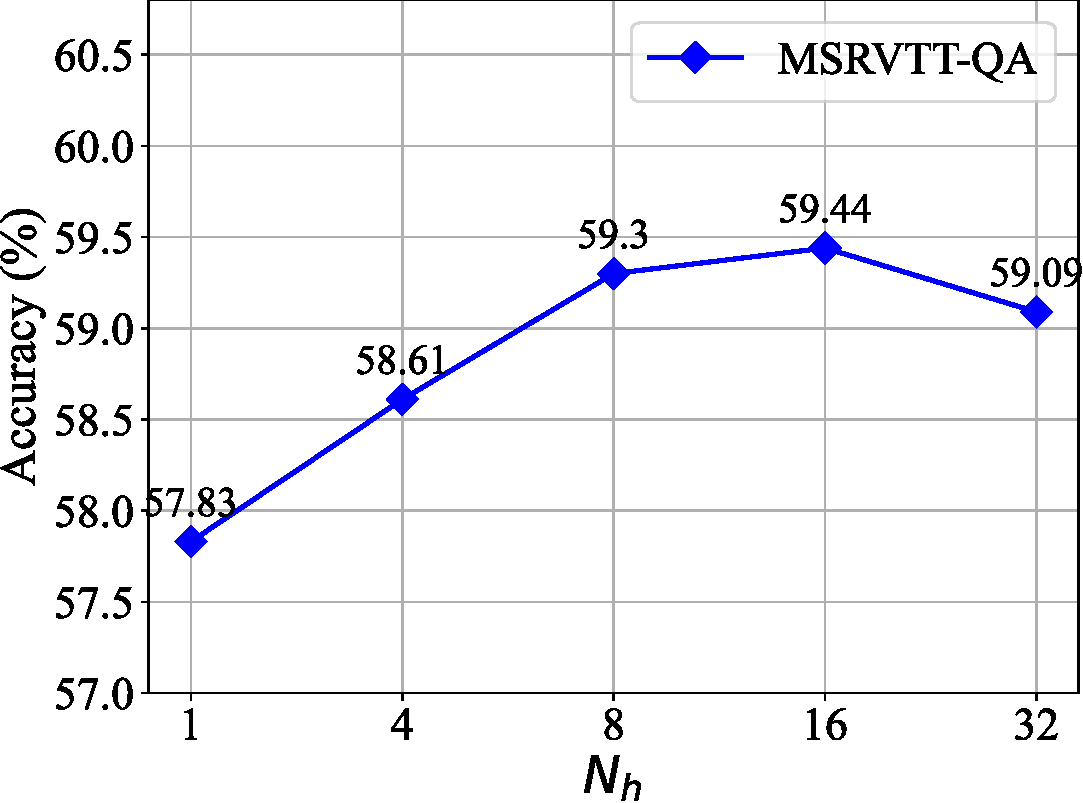
\includegraphics[height=5.5cm]{figure/c2_msrvtt_qa.pdf}
\subcaption{MSRVTT-QA}
\end{subfigure}
\begin{subfigure}[b]{0.49\linewidth}
\centering
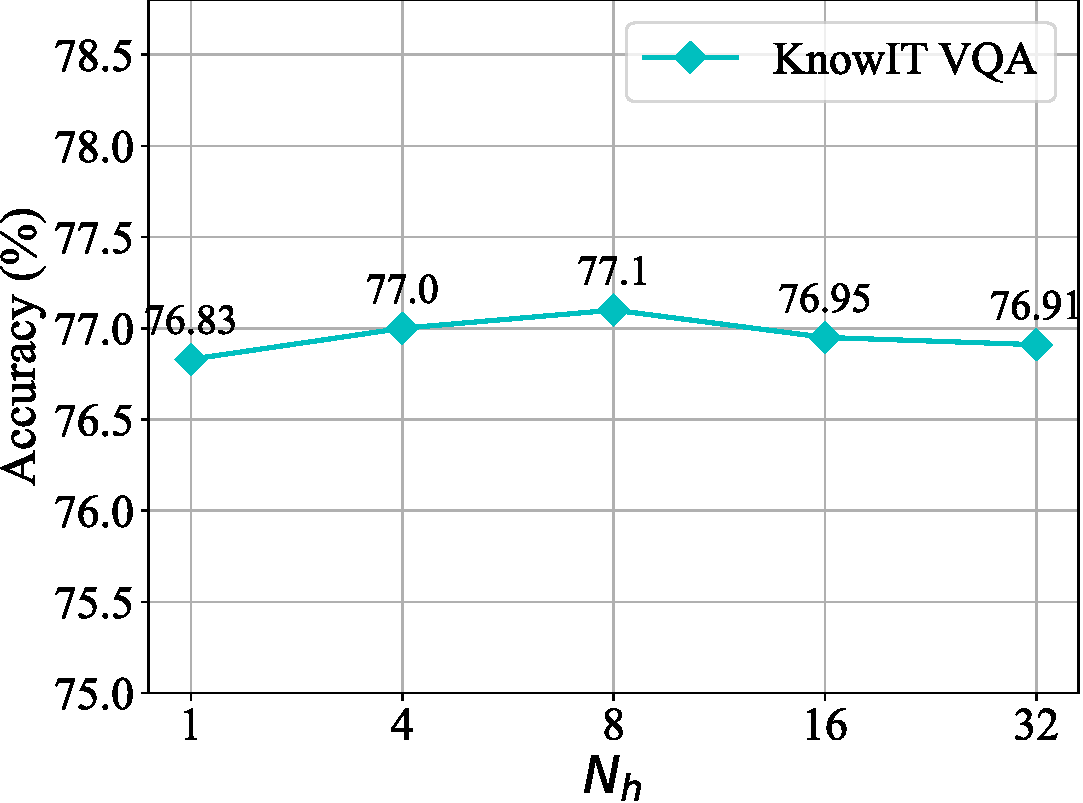
\includegraphics[height=5.5cm]{figure/c2_knowit_vqa.pdf}
\subcaption{KnowIT VQA}
\end{subfigure}
\caption{在MSRVTT-QA和KnowIT VQA数据集上不同$N_h$数值下LiVLR的性能}
\label{fig:c2_vis_param}
\end{figure}
% ********************************************************************

\subsubsection{多粒度视觉和语言表征对LiVLR的影响}
LiVLR利用具有相似结构的视觉编码器和语言编码器编码视频中的视觉和语言内容,这在一定程度上保证了从不同模态中获得的全局(细粒度)表征处于相同的语义水平。
为了分析多粒度视觉和语言表征的影响,本章首先考虑以下两组种对比:
$\blacktriangleright$ 表~\ref{tab:c2_abl_comps} (\#9 vs. \#1 vs. \#3)和$\blacktriangleright$ 表~\ref{tab:c2_abl_comps} (\#10 vs. \#2 vs. \#4)。本章从表中实验结果发现考虑多粒度视觉语言表征(\#9和\#10)时,LiVLR的性能显著地优于仅使用单一视觉(\#1和\#2)或单一语言表征(\#3和\#4)时。
然后,本章考虑另外的两组对比:$\blacktriangleright$ 表~\ref{tab:c2_abl_comps} (\#9 vs. \#5 vs. \#7)和$\blacktriangleright$ 表~\ref{tab:c2_abl_comps} (\#10 vs. \#6 vs. \#8)。类似地,本章也可以观察到考虑多粒度视觉语言表征(\#9和\#10)时,LiVLR的性能显著地优于仅使用全局(\#5和\#6)或者细粒度(\#7和\#8)表征时。
最后,为了进一步验证多粒度视觉和语言表征,特别是细粒度视觉和语言表征的优越性,本章进行了以下实验:$\blacktriangleright$ 使用一个两层的全连接网络代替视觉编码器和语言编码器中的图神经网络。表~\ref{tab:c2_abl_GCN2FC} 中的实验结果表明获得视觉对象或语言成分之间细粒度的视觉或语言表征对LiVLR也很重要。



\subsubsection{超参的影响}
为了进行更详细的参数分析,本章考虑公式~(\refeq{eq:alpha_ij})中的关键参数$N_h$。该参数直接影响表征整合方法DaVL的性能。具体来说,本章考虑以下设置,即,$N_h = 1, 4, 8, 16, 32$。
从图~\ref{fig:c2_vis_param}的实验结果本章可以观察到,与整体性能的提高相比,使用不同$N_h$的LiVLR的性能波动很小,表明本章的方法对超参数$N_h$是鲁棒的。


\xsubsection{定性实验}{Qualitative Experiment}

% % ********************************************************************
\begin{figure}[!t]
\vspace{-3mm}
\begin{subfigure}[b]{1.0\textwidth}
\centering
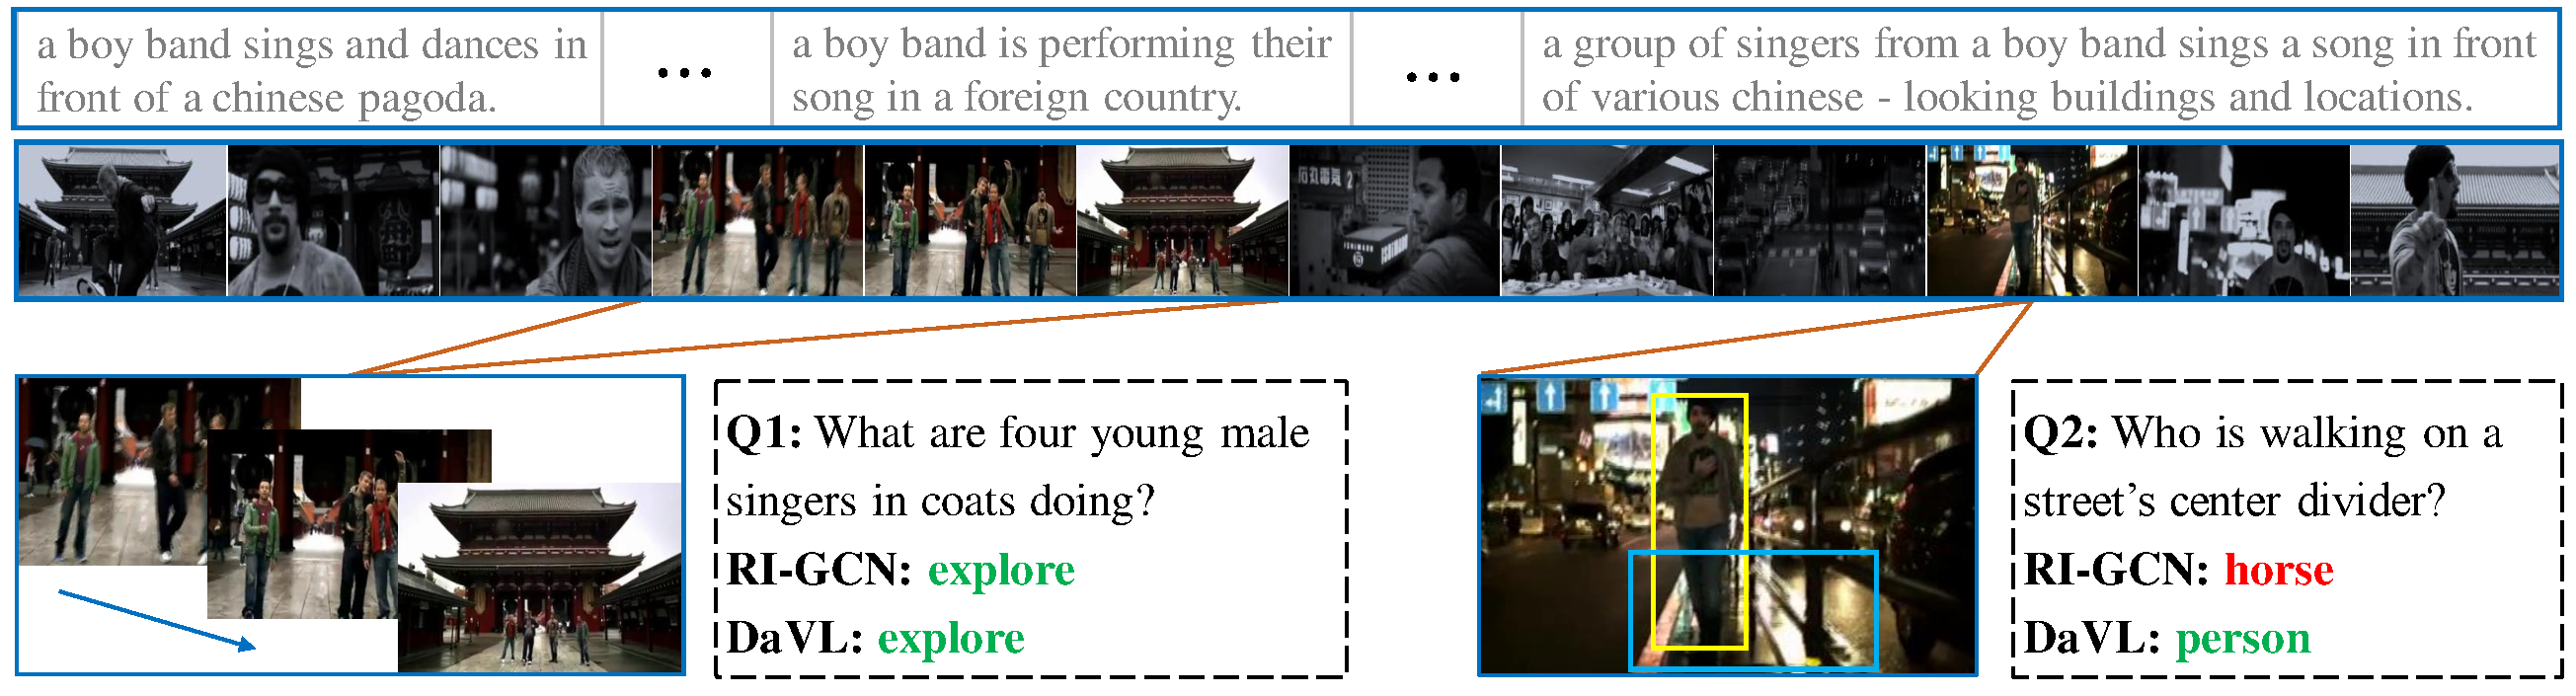
\includegraphics[width=0.98\linewidth]{figure/c2_vis_a.pdf}
\subcaption{回答问题Q1和Q2需要理解该视频片段中全局和细粒度的视觉内容
}
\label{fig:c2_vis_correct_1}
\end{subfigure}
\begin{subfigure}[b]{1.0\textwidth}
\centering
\vspace{-1mm}
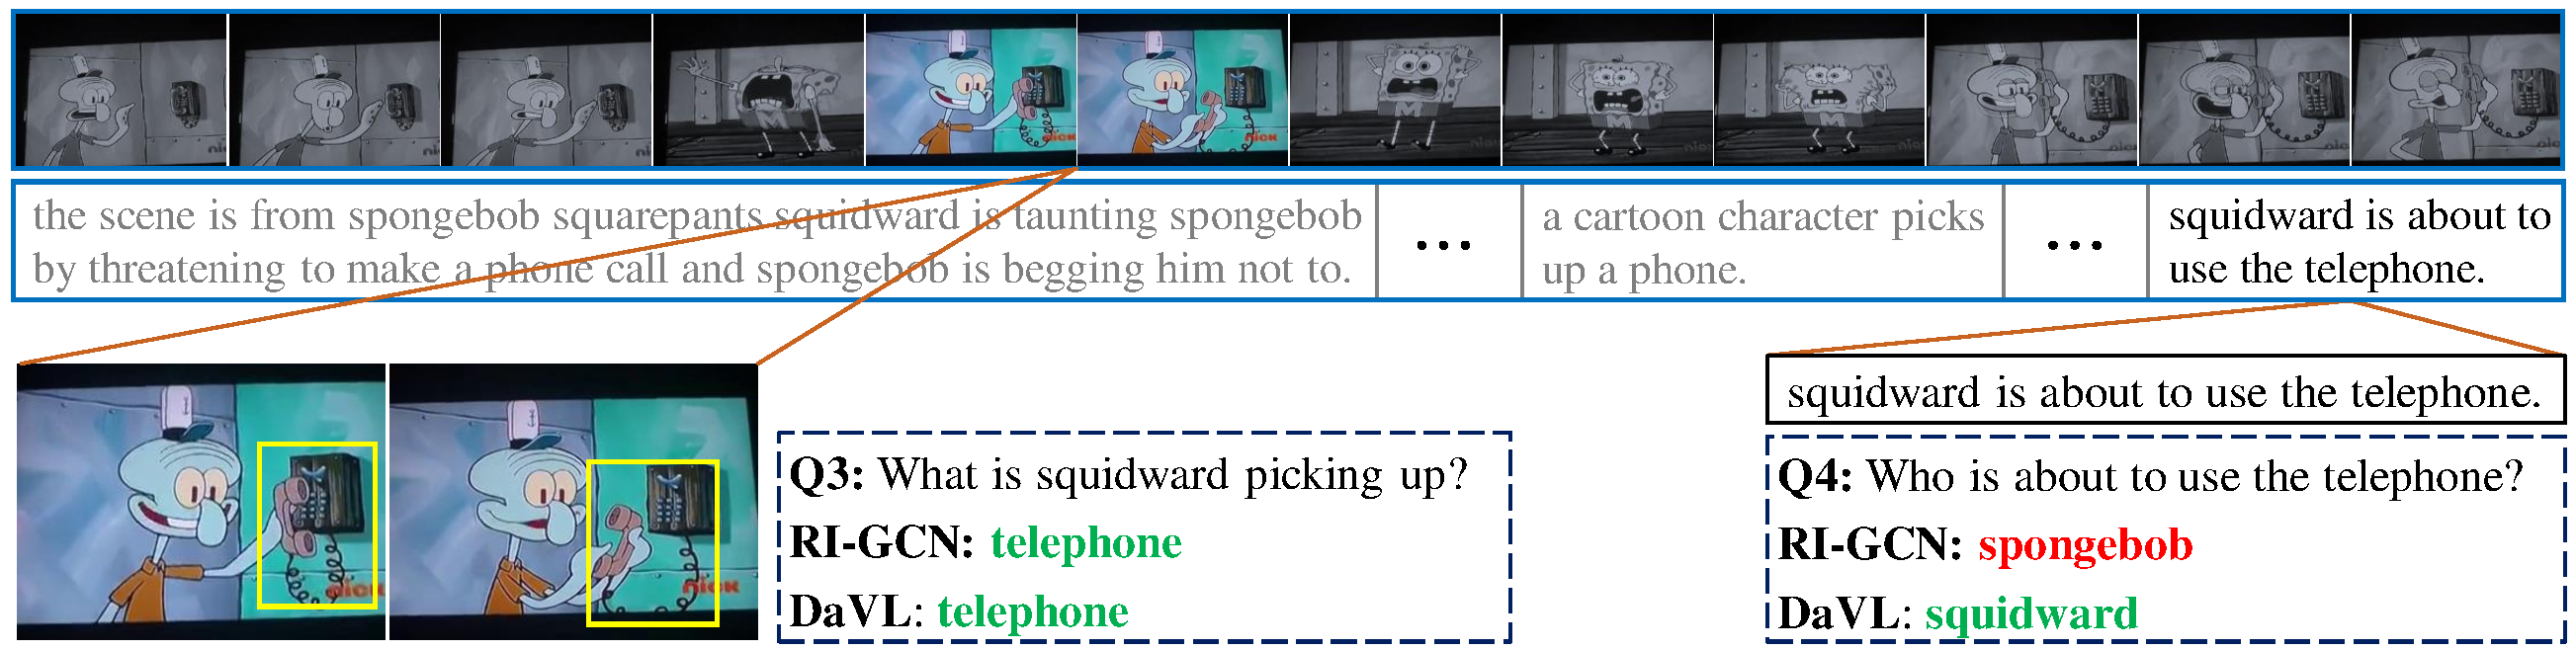
\includegraphics[width=0.98\linewidth]{figure/c2_vis_b.pdf}
\subcaption{回答问题Q3和Q4需要理解该视频片段中的视觉和语言内容}
\label{fig:c2_vis_correct_2}
\end{subfigure}
\vspace{-6mm}
\caption{在MSRVTT-QA数据集上的可视化举例
}
\end{figure}
% % ********************************************************************

\subsubsection{定性实验结果}
为了定性地评估本章节所提出的表征整合方法DaVL的有效性,本章可视化了MSRVTT-QA数据集上一些答案预测结果。
在图~\ref{fig:c2_vis_correct_1}中,本章展示了对应于同一视频片段的两个问题。具体来说,回答问题Q1需要理解该视频片段中描述的整体事件;回答Q2则需要理解该视频片段中细粒度的视觉内容。
实验结果显示使用RI-GCN和DaVL均能正确回答问题Q1,但使用RI-GCN并没有正确回答问题Q2。
在图~\ref{fig:c2_vis_correct_2}中,回答问题Q3需要理解视频片段中的视觉内容;回答问题Q4则需要理解该视频片段对应的语言描述的内容。
实验结果显示尽管使用RI-GCN和DaVL均可以正确回答与视觉内容有关的问题Q3,但使用RI-GCN却不能回答与语言内容有关的问题Q4。
以上两组对比表明了在基于图的表征整合中考虑表征多样性的重要性。
兼顾表征的多样性在一定程度上可以促进视频问答系统自适应地选择给定问题所需的表征,进而促进视频问答系统灵活地应对各种各样的问题。



\subsubsection{典型失败案例分析}
图~\ref{fig:c2_vis_error} 展示了在MSRVTT-QA数据集上的两种典型失败案例。
具体来说,
图~\ref{fig:c2_vis_error_1} 显示在表征整合时DaVL使用了多粒度语言表征,本章提出的LiVLR反而会错误地回答这个问题。该案例表明,在回答只与视觉内容有关的问题时,可学习的索引嵌入可能不足以让DaVL选择所需的视觉表征而忽略不相关的语言表征。
在图~\ref{fig:c2_vis_error_2} 中,使用基于图的表征整合方法(即RI-GCN和DaVL)未能正确回答该问题,反而是使用更简单的表征整合方法(即RI-Concat和RI-AT)正确地回答了该问题。
该案例表明,在回答语义复杂的问题时,基于图的表征整合方法有时可能会失去节点(即不同类型的表征)间的辨别性,阐述了使用基于图的表征整合方法固有的局限性。


% ********************************************************************
\begin{figure}[!t]
% \centering
\begin{subfigure}[b]{0.42\textwidth}
\centering
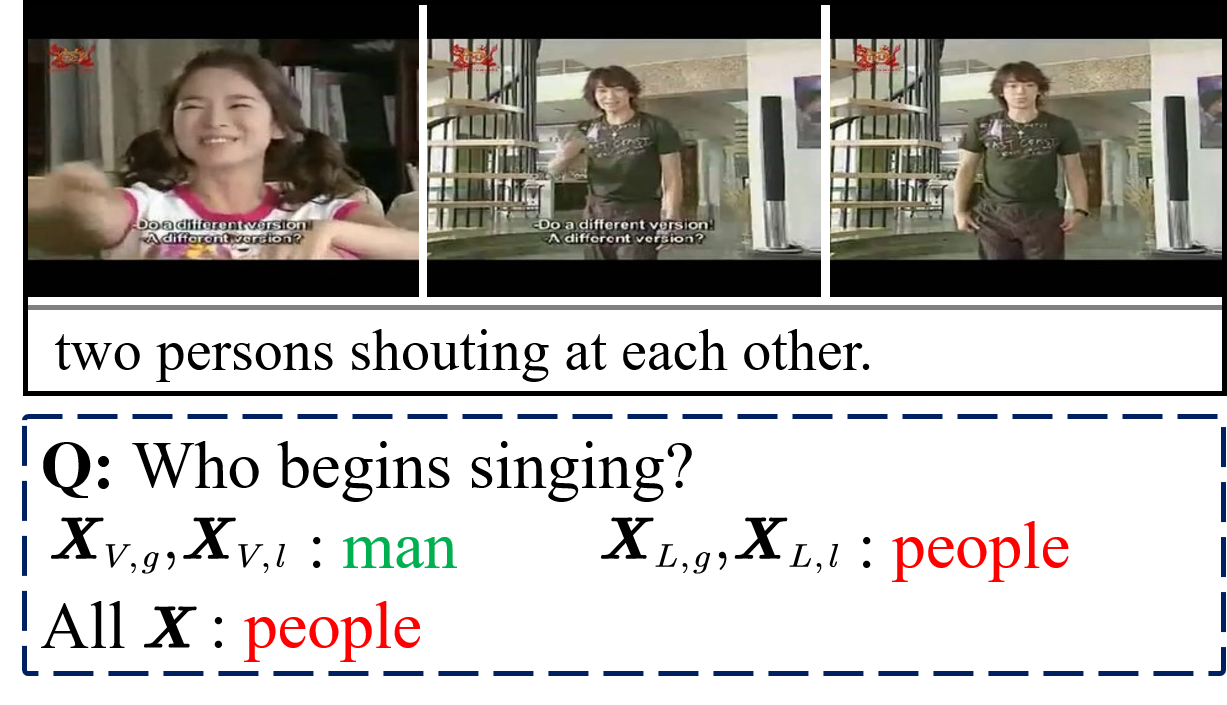
\includegraphics[height=3.7cm]{figure/c2_e1.png}
\subcaption{语言表征导致的错误}
\label{fig:c2_vis_error_1}
\end{subfigure}
\begin{subfigure}[b]{0.56\textwidth}
\centering
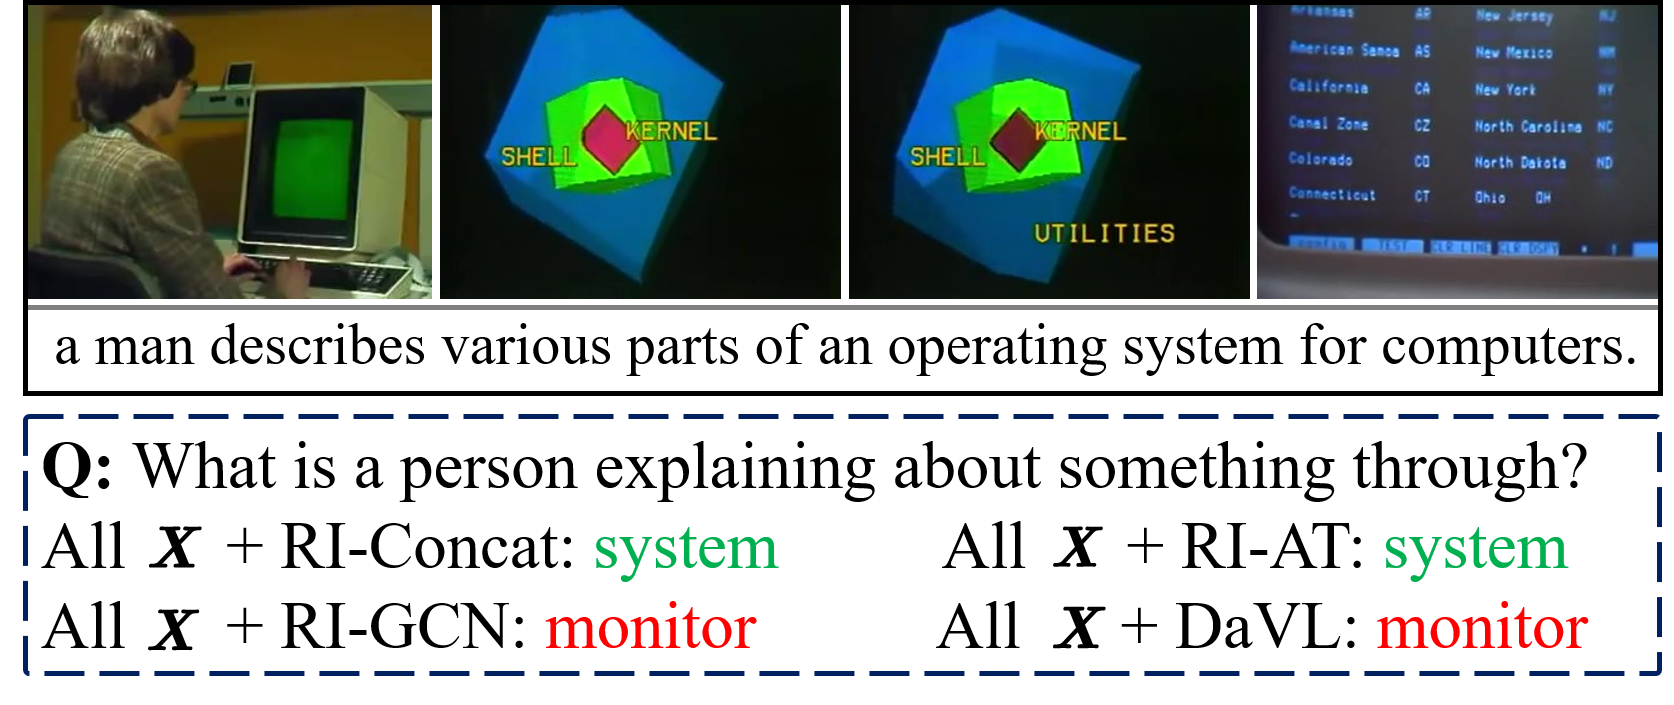
\includegraphics[height=3.7cm]{figure/c2_e2.png}
\subcaption{图的表征整合方法导致的错误}
\label{fig:c2_vis_error_2}
\end{subfigure}
\caption{在MSRVTT-QA数据集上的典型失败案例}
\label{fig:c2_vis_error}
\end{figure}
% ********************************************************************


% **************************************************************************
\xsection{本章小结}{Summary}
本章提出了基于多粒度视觉语言推理的视频问答方法LiVLR。
该方法首先使用基于图的视觉编码器和语言编码器在不同尺度上对视频的视觉和语言内容进行同层次的编码,来获得多粒度的视觉和语言表征;
然后利用本章提出的多样性感知的视觉语言推理模块在兼顾表征多样性的同时整合所获得的表征,生成联合表征来进行答案预测。
LiVLR是轻量级的,在开放式和多选式的视频问答数据集上均表现出了性能优势。
在未来,我们的目标是探索一种全新的语言编码方法,它可以有效地对给定的问题进行多尺度的编码,更灵活地与视频内容进行交互。



\clearpage
